%!TeX root=../wowtop.tex

\ArtChapter[Dead London]{25head}

\begin{figure}[p]
\centering

\includegraphics[width=\linewidth]{25deadlondon}
\caption{A city condemned and derelict}
\end{figure}

\lettrine[lines=4,findent=2pt]{A}{fter} I had parted from the artilleryman, I went down the hill, and by the High Street across the bridge to Fulham. The red weed was tumultuous at that time, and nearly choked the bridge roadway; but its fronds were already whitened in patches by the spreading disease that presently removed it so swiftly.

At the corner of the lane that runs to Putney Bridge station I found a man lying. He was as black as a sweep with the black dust, alive, but helplessly and speechlessly drunk. I could get nothing from him but curses and furious lunges at my head. I think I should have stayed by him but for the brutal expression of his face.

\begin{figure}[tb!]
\centering
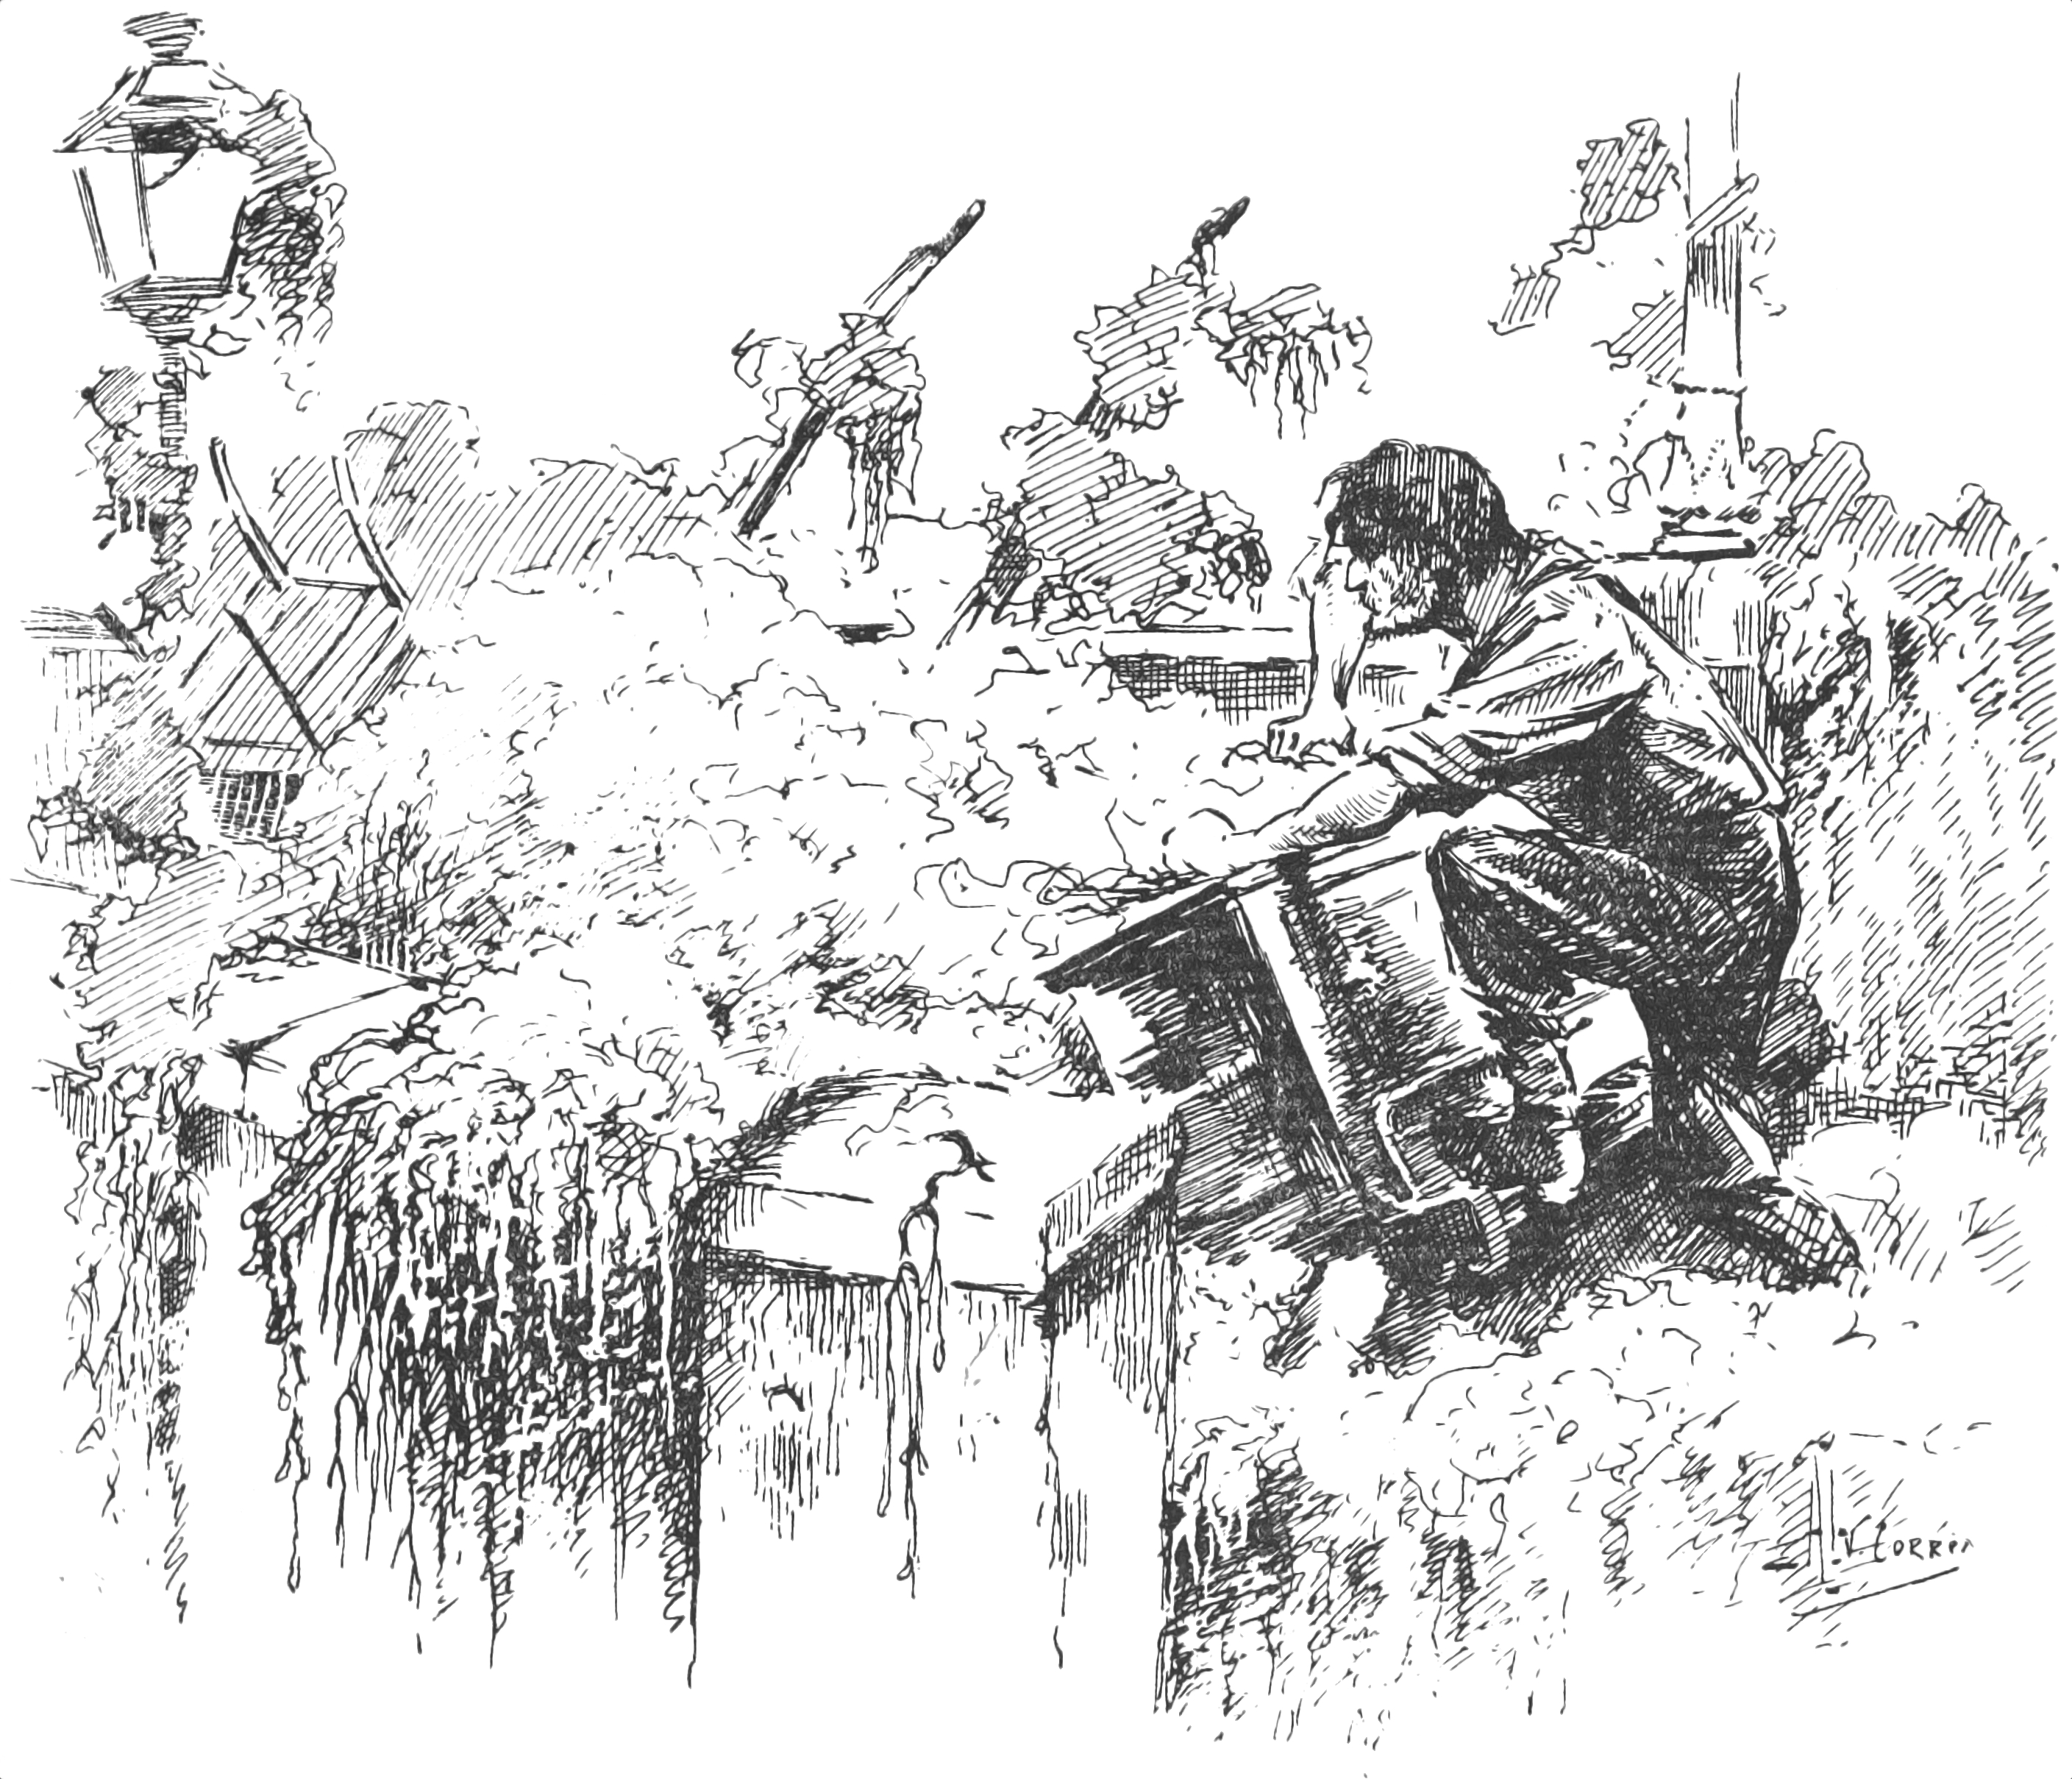
\includegraphics[width=.8\textwidth]{25overgrown}
\end{figure}

There was black dust along the roadway from the bridge onwards, and it grew thicker in Fulham. The streets were horribly quiet. I got food—sour, hard, and mouldy, but quite eatable—in a baker's shop here. Some way towards Walham Green the streets became clear of powder, and I passed a white terrace of houses on fire; the noise of the burning was an absolute relief. Going on towards Brompton, the streets were quiet again.

Here I came once more upon the black powder in the streets and upon dead bodies. I saw altogether about a dozen in the length of the Fulham Road. They had been dead many days, so that I hurried quickly past them. The black powder covered them over, and softened their outlines. One or two had been disturbed by dogs.



Where there was no black powder, it was curiously like a Sunday in the City, with the closed shops, the houses locked up and the blinds drawn, the desertion, and the stillness. In some places plunderers had been at work, but rarely at other than the provision and wine shops. A jeweller's window had been broken open in one place, but apparently the thief had been disturbed, and a number of gold chains and a watch lay scattered on the pavement. I did not trouble to touch them. Farther on was a tattered woman in a heap on a doorstep; the hand that hung over her knee was gashed and bled down her rusty brown dress, and a smashed magnum of champagne formed a pool across the pavement. She seemed asleep, but she was dead.

The farther I penetrated into London, the profounder grew the stillness. But it was not so much the stillness of death—it was the stillness of suspense, of expectation. At any time the destruction that had already singed the northwestern borders of the metropolis, and had annihilated Ealing and Kilburn, might strike among these houses and leave them smoking ruins. It was a city condemned and derelict\textellipsis

In South Kensington the streets were clear of dead and of black powder. It was near South Kensington that I first heard the howling. It crept almost imperceptibly upon my senses. It was a sobbing alternation of two notes, »Ulla, ulla, ulla, ulla,« keeping on perpetually. When I passed streets that ran northward it grew in volume, and houses and buildings seemed to deaden and cut it off again. It came in a full tide down Exhibition Road. I stopped, staring towards Kensington Gardens, wondering at this strange, remote wailing. It was as if that mighty desert of houses had found a voice for its fear and solitude.

»Ulla, ulla, ulla, ulla,« wailed that superhuman note—great waves of sound sweeping down the broad, sunlit roadway, between the tall buildings on each side. I turned northwards, marvelling, towards the iron gates of Hyde Park. I had half a mind to break into the Natural History Museum and find my way up to the summits of the towers, in order to see across the park. But I decided to keep to the ground, where quick hiding was possible, and so went on up the Exhibition Road. All the large mansions on each side of the road were empty and still, and my footsteps echoed against the sides of the houses. At the top, near the park gate, I came upon a strange sight—a bus overturned, and the skeleton of a horse picked clean. I puzzled over this for a time, and then went on to the bridge over the Serpentine. The voice grew stronger and stronger, though I could see nothing above the housetops on the north side of the park, save a haze of smoke to the northwest.

\begin{figure}[p]
\centering
\includegraphics[width=\linewidth]{25citynoir}
\caption{My footsteps echoed against the sides of the houses}
\end{figure}

»Ulla, ulla, ulla, ulla,« cried the voice, coming, as it seemed to me, from the district about Regent's Park. The desolating cry worked upon my mind. The mood that had sustained me passed. The wailing took possession of me. I found I was intensely weary, footsore, and now again hungry and thirsty.

It was already past noon. Why was I wandering alone in this city of the dead? Why was I alone when all London was lying in state, and in its black shroud? I felt intolerably lonely. My mind ran on old friends that I had forgotten for years. I thought of the poisons in the chemists' shops, of the liquors the wine merchants stored; I recalled the two sodden creatures of despair, who so far as I knew, shared the city with myself\textellipsis

I came into Oxford Street by the Marble Arch, and here again were black powder and several bodies, and an evil, ominous smell from the gratings of the cellars of some of the houses. I grew very thirsty after the heat of my long walk. With infinite trouble I managed to break into a public-house and get food and drink. I was weary after eating, and went into the parlour behind the bar, and slept on a black horsehair sofa I found there.

I awoke to find that dismal howling still in my ears, »Ulla, ulla, ulla, ulla.« It was now dusk, and after I had routed out some biscuits and a cheese in the bar—there was a meat safe, but it contained nothing but maggots—I wandered on through the silent residential squares to Baker Street—Portman Square is the only one I can name—and so came out at last upon Regent's Park. And as I emerged from the top of Baker Street, I saw far away over the trees in the clearness of the sunset the hood of the Martian giant from which this howling proceeded. I was not terrified. I came upon him as if it were a matter of course. I watched him for some time, but he did not move. He appeared to be standing and yelling, for no reason that I could discover.

\begin{wrapfigure}{O}{0.4\textwidth}
\centering
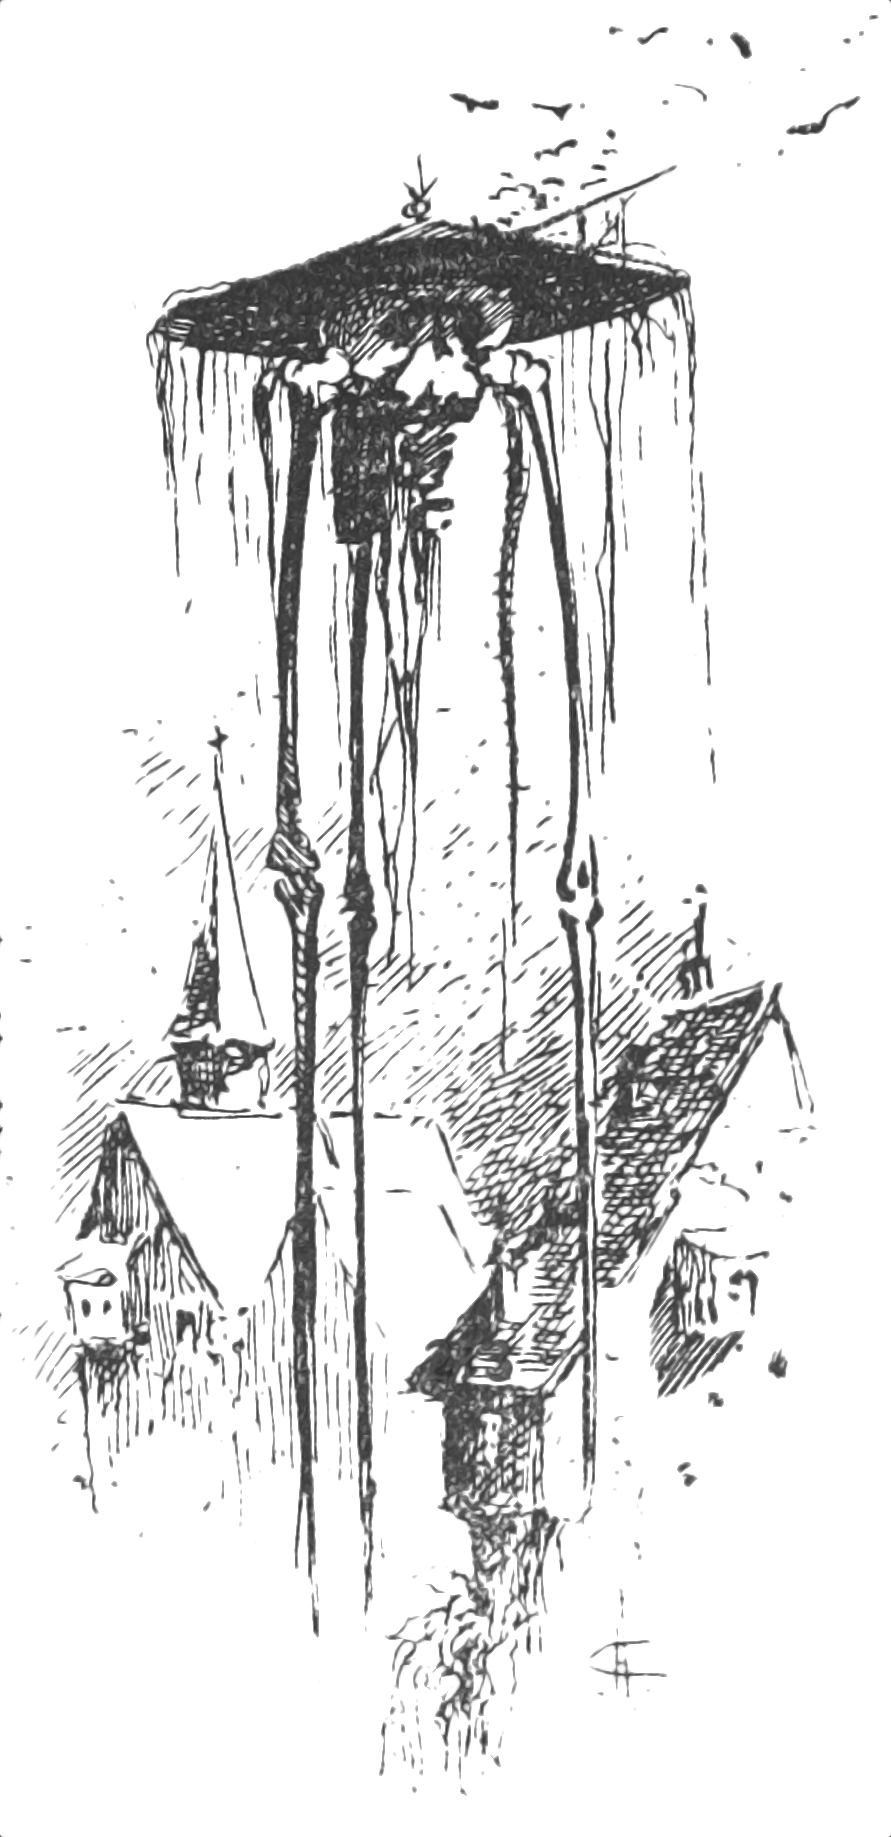
\includegraphics[width=0.4\textwidth]{25citytripod}
\end{wrapfigure}

I tried to formulate a plan of action. That perpetual sound of »Ulla, ulla, ulla, ulla,« confused my mind. Perhaps I was too tired to be very fearful. Certainly I was more curious to know the reason of this monotonous crying than afraid. I turned back away from the park and struck into Park Road, intending to skirt the park, went along under the shelter of the terraces, and got a view of this stationary, howling Martian from the direction of St~John's Wood. A couple of hundred yards out of Baker Street I heard a yelping chorus, and saw, first a dog with a piece of putrescent red meat in his jaws coming headlong towards me, and then a pack of starving mongrels in pursuit of him. He made a wide curve to avoid me, as though he feared I might prove a fresh competitor. As the yelping died away down the silent road, the wailing sound of »Ulla, ulla, ulla, ulla,« reasserted itself.

I came upon the wrecked handling-machine halfway to St~John's Wood station. At first I thought a house had fallen across the road. It was only as I clambered among the ruins that I saw, with a start, this mechanical Samson lying, with its tentacles bent and smashed and twisted, among the ruins it had made. The forepart was shattered. It seemed as if it had driven blindly straight at the house, and had been overwhelmed in its overthrow. It seemed to me then that this might have happened by a handling-machine escaping from the guidance of its Martian. I could not clamber among the ruins to see it, and the twilight was now so far advanced that the blood with which its seat was smeared, and the gnawed gristle of the Martian that the dogs had left, were invisible to me.

\begin{figure}[p]
\centering
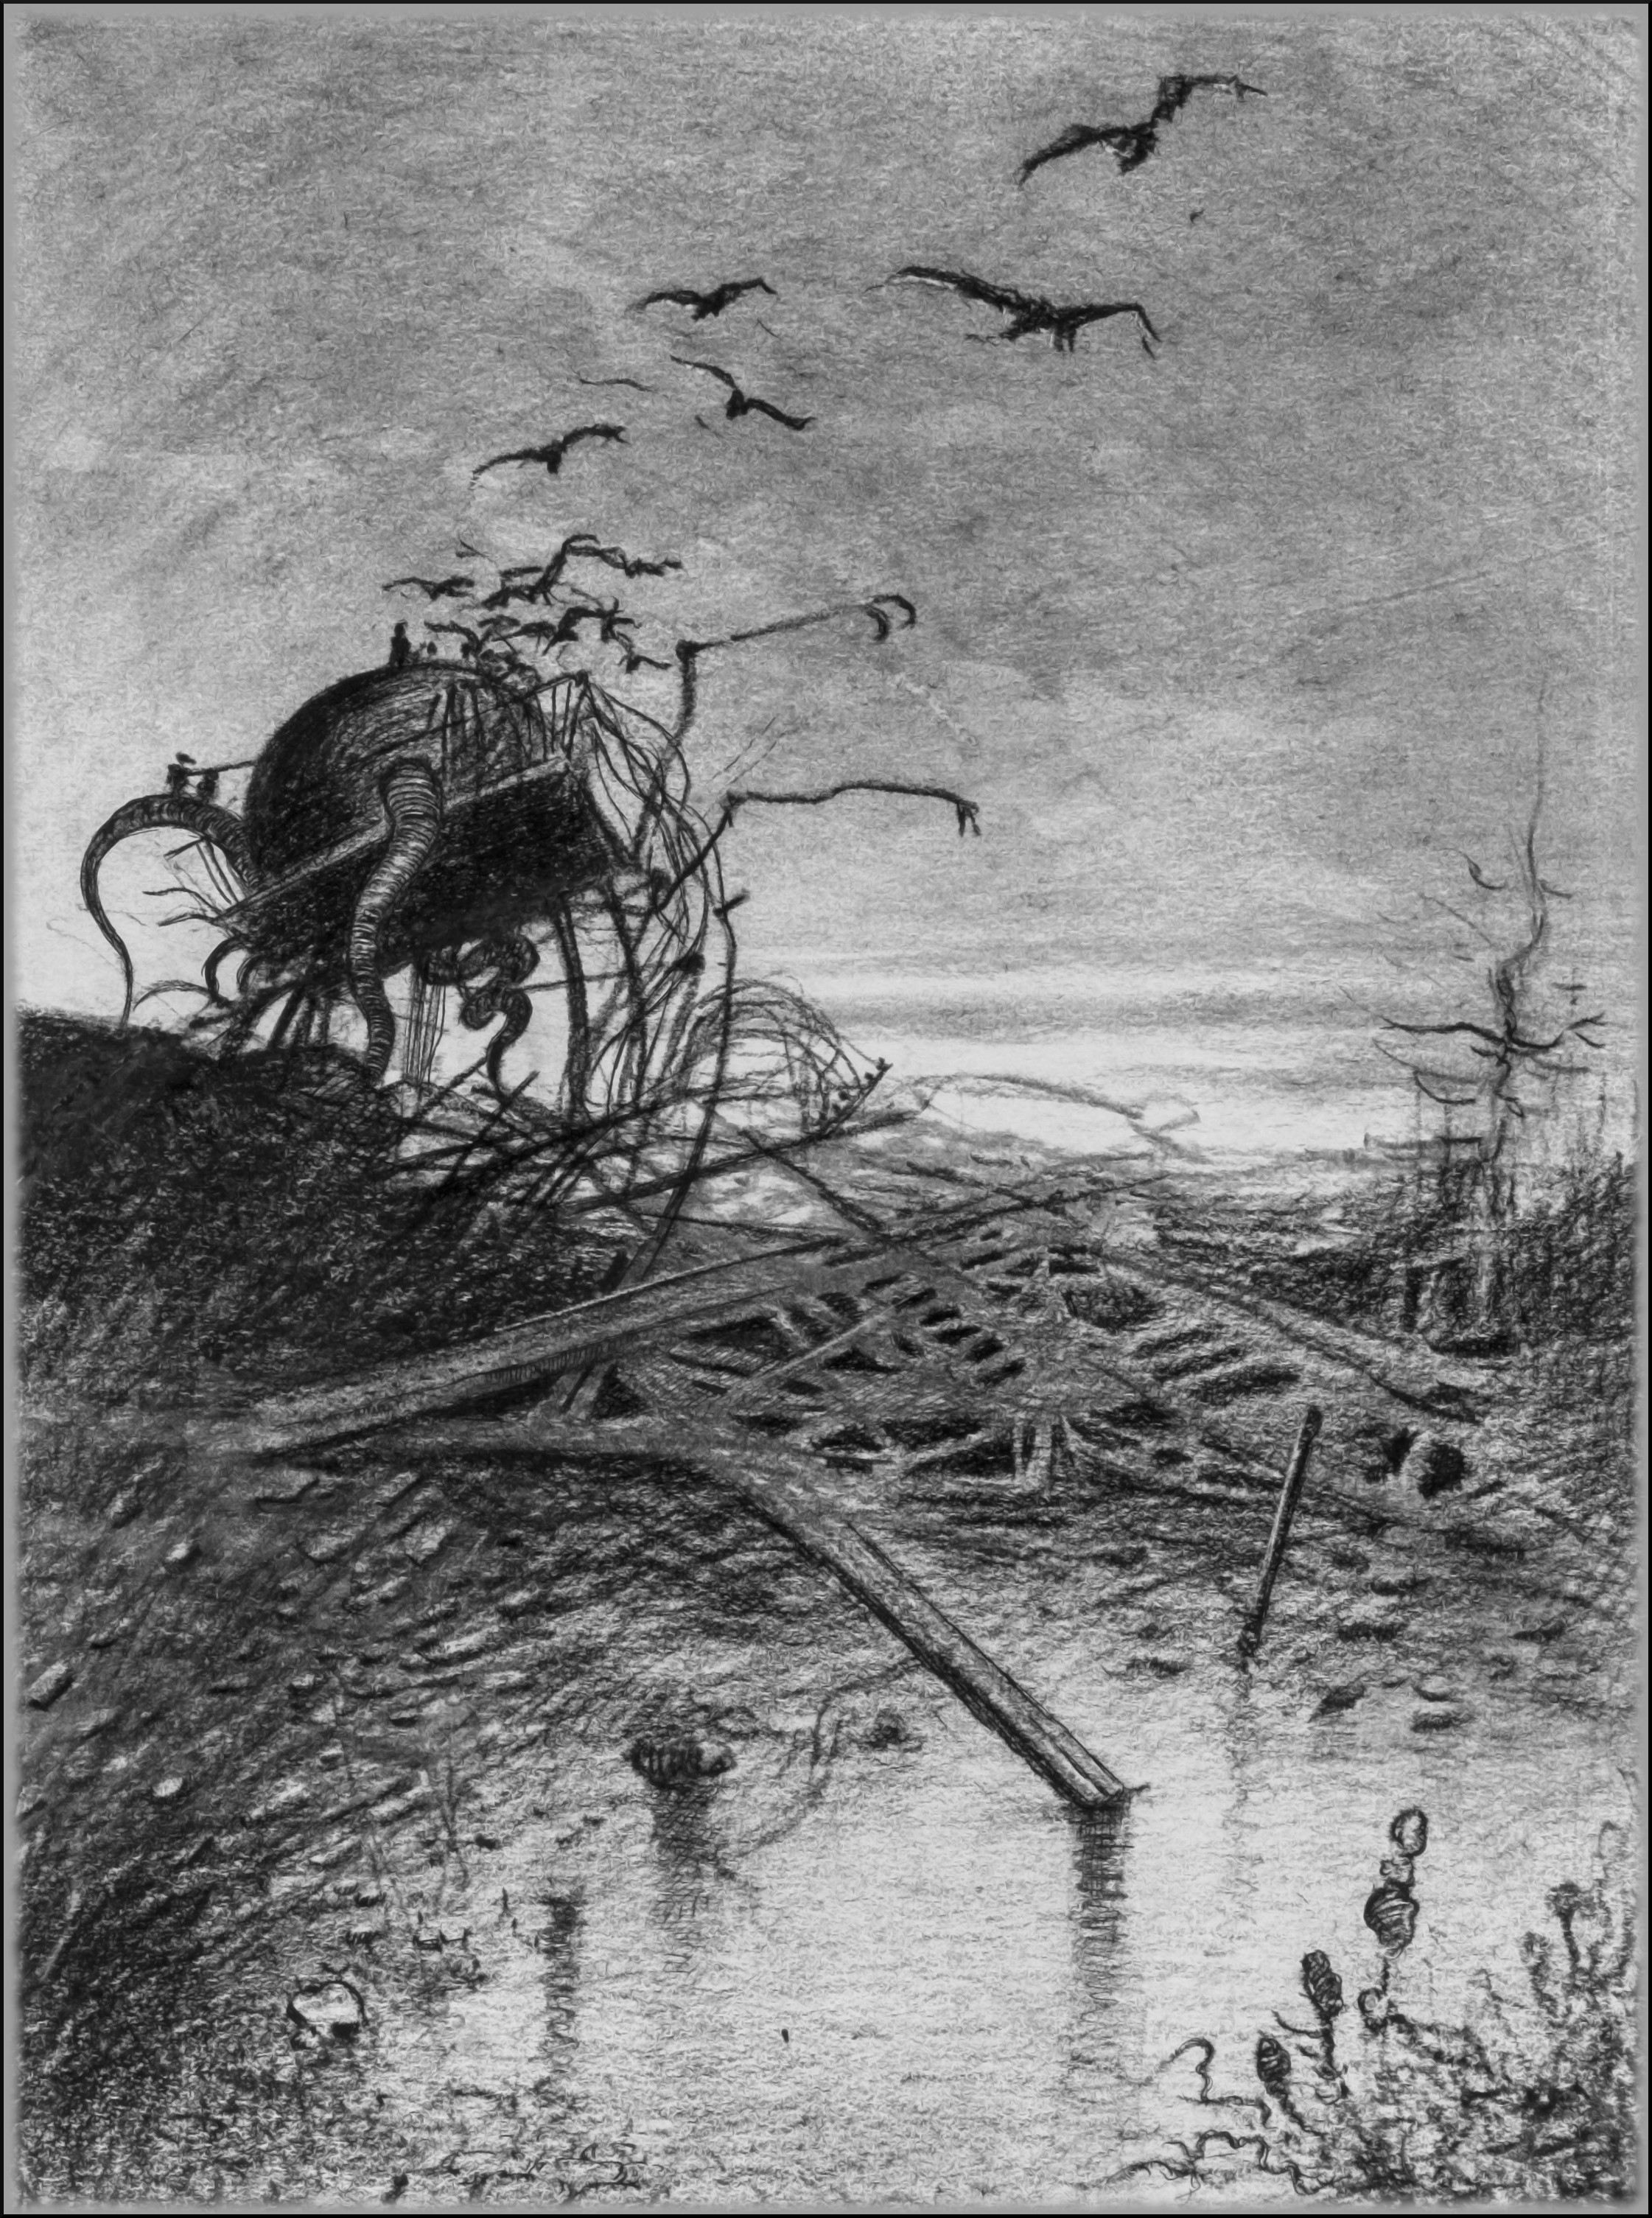
\includegraphics[width=\linewidth]{25samson}
\caption{This mechanical Samson lying among the ruins it had made}
\end{figure}

Wondering still more at all that I had seen, I pushed on towards Primrose Hill. Far away, through a gap in the trees, I saw a second Martian, as motionless as the first, standing in the park towards the Zoological Gardens, and silent. A little beyond the ruins about the smashed handling-machine I came upon the red weed again, and found the Regent's Canal, a spongy mass of dark-red vegetation.

As I crossed the bridge, the sound of »Ulla, ulla, ulla, ulla,« ceased. It was, as it were, cut off. The silence came like a thunderclap.

The dusky houses about me stood faint and tall and dim; the trees towards the park were growing black. All about me the red weed clambered among the ruins, writhing to get above me in the dimness. Night, the mother of fear and mystery, was coming upon me. But while that voice sounded the solitude, the desolation, had been endurable; by virtue of it London had still seemed alive, and the sense of life about me had upheld me. Then suddenly a change, the passing of something—I knew not what—and then a stillness that could be felt. Nothing but this gaunt quiet.

London about me gazed at me spectrally. The windows in the white houses were like the eye sockets of skulls. About me my imagination found a thousand noiseless enemies moving. Terror seized me, a horror of my temerity. In front of me the road became pitchy black as though it was tarred, and I saw a contorted shape lying across the pathway. I could not bring myself to go on. I turned down St~John's Wood Road, and ran headlong from this unendurable stillness towards Kilburn. I hid from the night and the silence, until long after midnight, in a cabmen's shelter in Harrow Road. But before the dawn my courage returned, and while the stars were still in the sky I turned once more towards Regent's Park. I missed my way among the streets, and presently saw down a long avenue, in the half-light of the early dawn, the curve of Primrose Hill. On the summit, towering up to the fading stars, was a third Martian, erect and motionless like the others.

\begin{figure}[p]
\centering
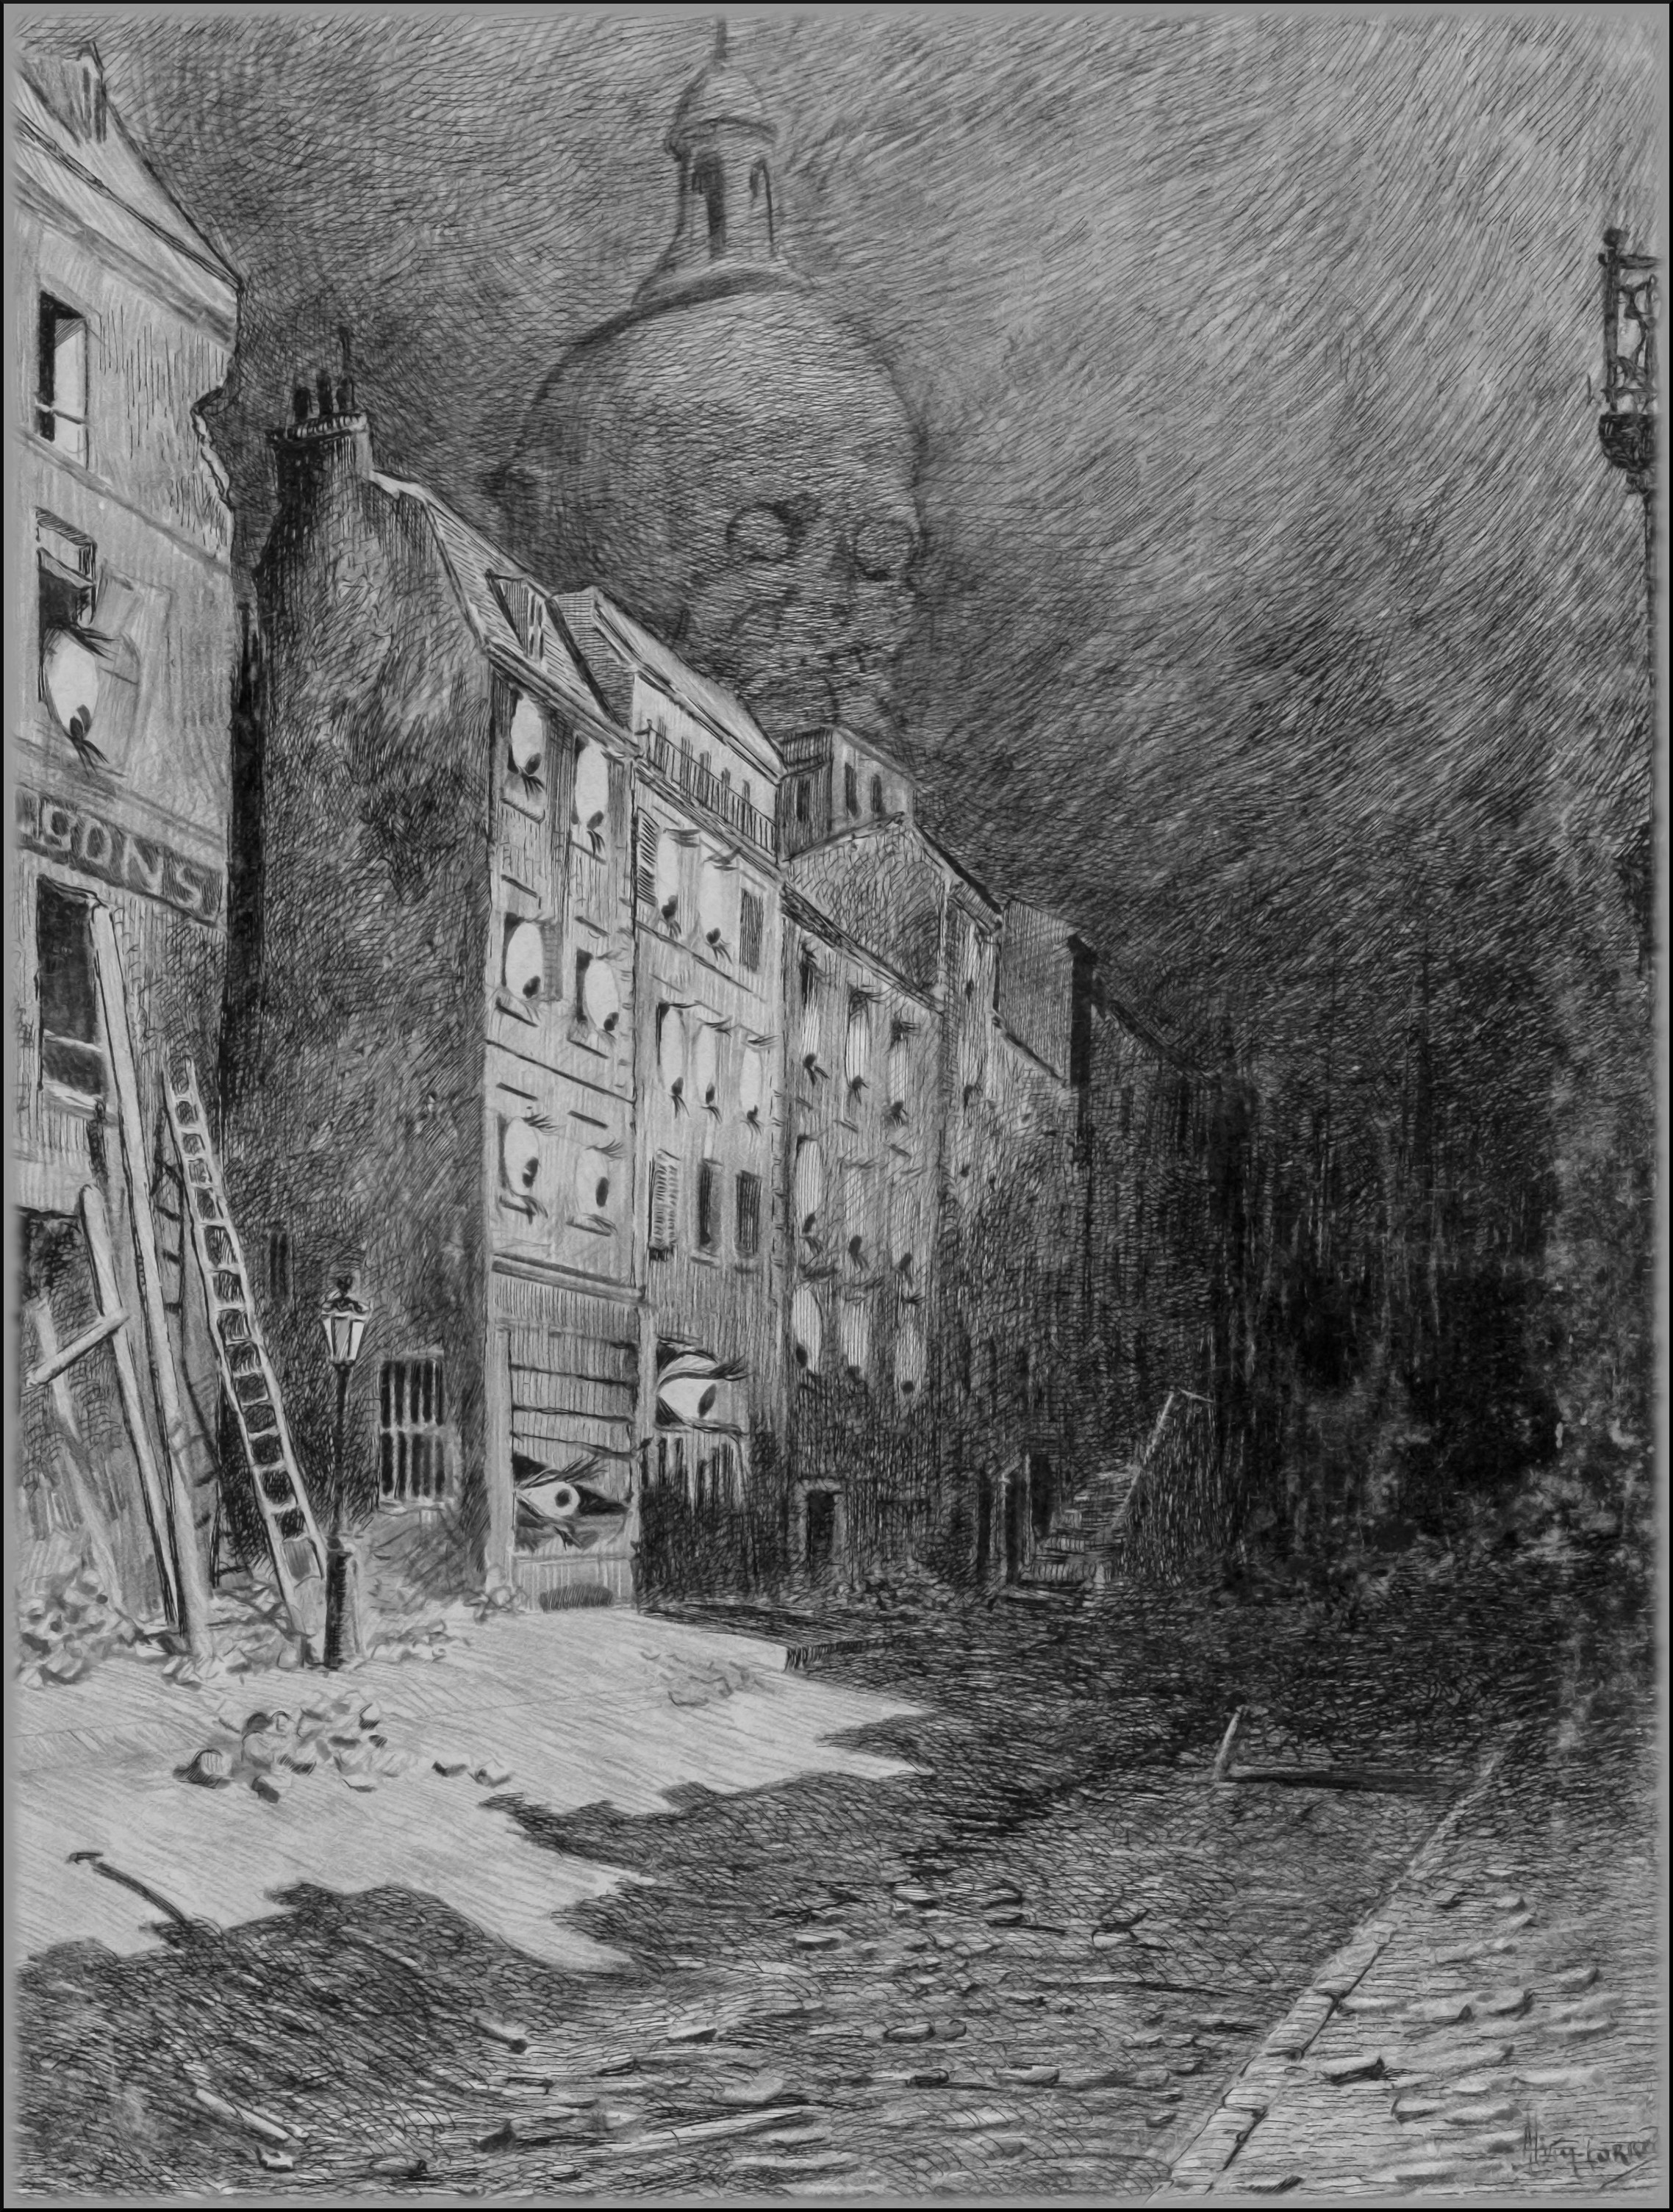
\includegraphics[width=\linewidth]{25spectrally}
\caption{London gazed at me spectrally}
\end{figure}

An insane resolve possessed me. I would die and end it. And I would save myself even the trouble of killing myself. I marched on recklessly towards this Titan, and then, as I drew nearer and the light grew, I saw that a multitude of black birds was circling and clustering about the hood. At that my heart gave a bound, and I began running along the road.

I hurried through the red weed that choked St~Edmund's Terrace (I waded breast-high across a torrent of water that was rushing down from the waterworks towards the Albert Road), and emerged upon the grass before the rising of the sun. Great mounds had been heaped about the crest of the hill, making a huge redoubt of it—it was the final and largest place the Martians had made—and from behind these heaps there rose a thin smoke against the sky. Against the sky line an eager dog ran and disappeared. The thought that had flashed into my mind grew real, grew credible. I felt no fear, only a wild, trembling exultation, as I ran up the hill towards the motionless monster. Out of the hood hung lank shreds of brown, at which the hungry birds pecked and tore.


In another moment I had scrambled up the earthen rampart and stood upon its crest, and the interior of the redoubt was below me. A mighty space it was, with gigantic machines here and there within it, huge mounds of material and strange shelter places. And scattered about it, some in their overturned war-machines, some in the now rigid handling-machines, and a dozen of them stark and silent and laid in a row, were the Martians—\textit{dead}!—slain by the putrefactive and disease bacteria against which their systems were unprepared; slain as the red weed was being slain; slain, after all man's devices had failed, by the humblest things that God, in his wisdom, has put upon this earth.

For so it had come about, as indeed I and many men might have foreseen had not terror and disaster blinded our minds. These germs of disease have taken toll of humanity since the beginning of things—taken toll of our prehuman ancestors since life began here. But by virtue of this natural selection of our kind we have developed resisting power; to no germs do we succumb without a struggle, and to many—those that cause putrefaction in dead matter, for instance—our living frames are altogether immune. But there are no bacteria in Mars, and directly these invaders arrived, directly they drank and fed, our microscopic allies began to work their overthrow. Already when I watched them they were irrevocably doomed, dying and rotting even as they went to and fro. It was inevitable. By the toll of a billion deaths man has bought his birthright of the earth, and it is his against all comers; it would still be his were the Martians ten times as mighty as they are. For neither do men live nor die in vain.



Here and there they were scattered, nearly fifty altogether, in that great gulf they had made, overtaken by a death that must have seemed to them as incomprehensible as any death could be. To me also at that time this death was incomprehensible. All I knew was that these things that had been alive and so terrible to men were dead. For a moment I believed that the destruction of Sennacherib had been repeated, that God had repented, that the Angel of Death had slain them in the night.

\begin{figure}[tbp]
\centering
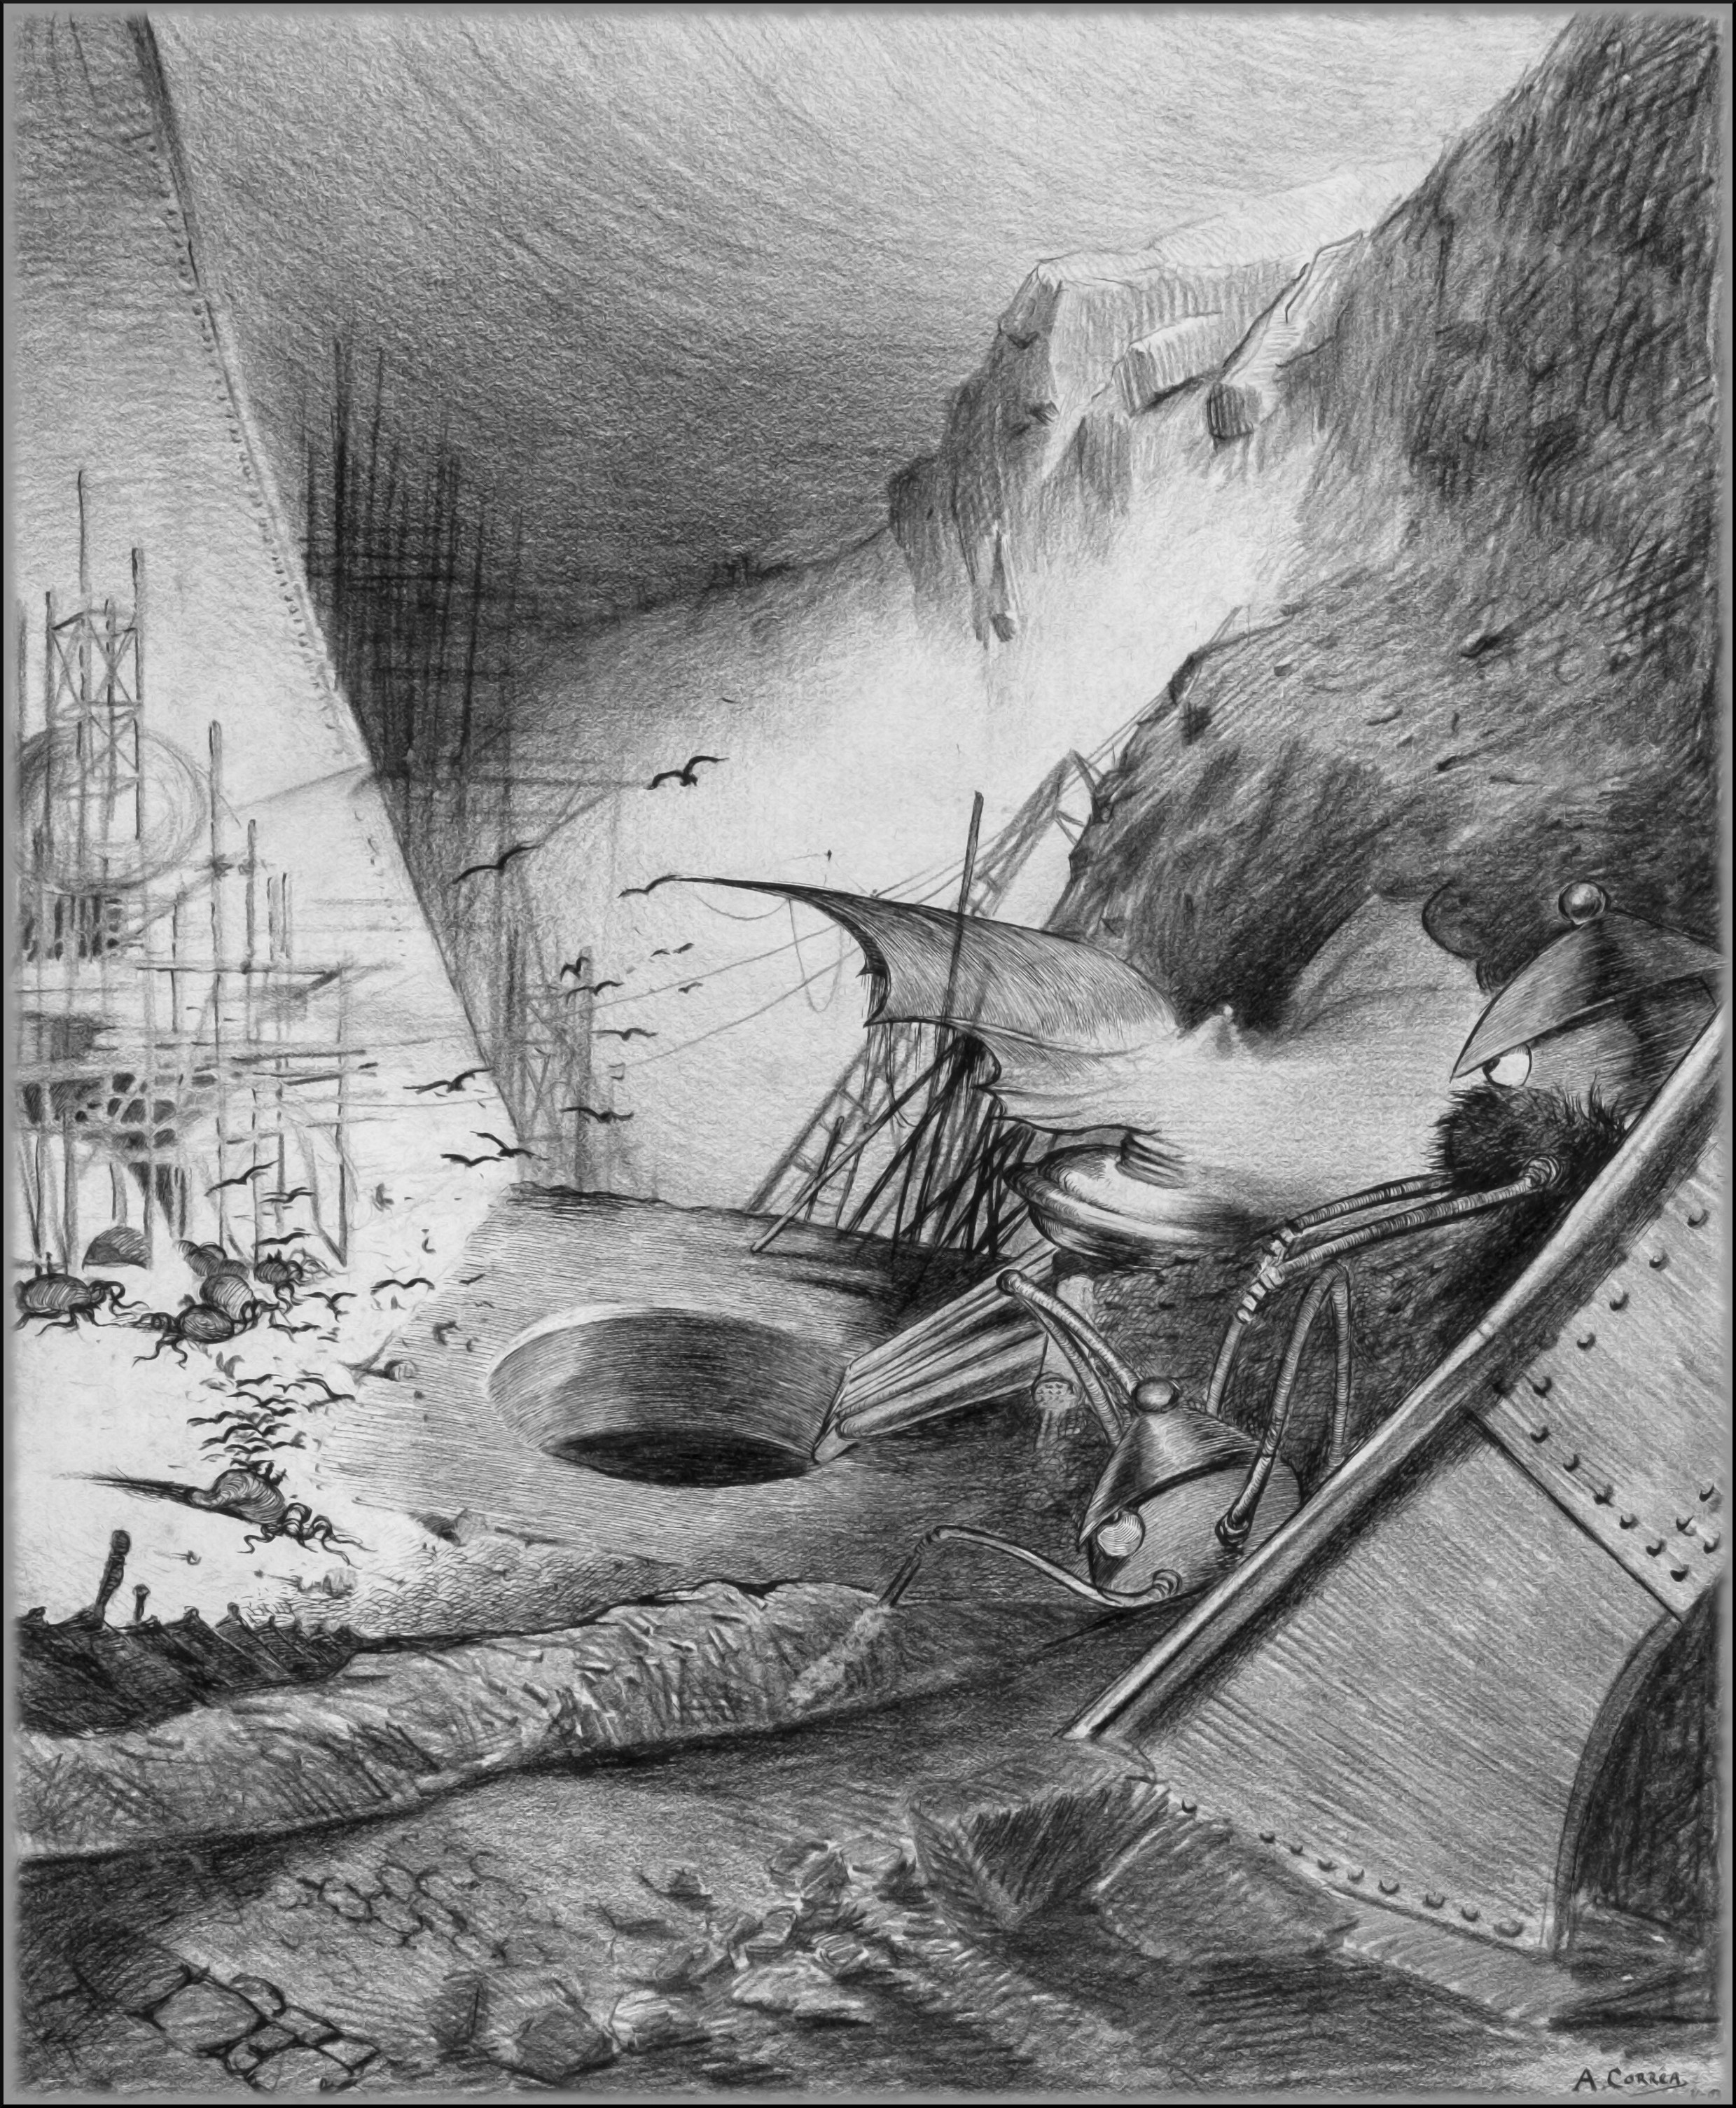
\includegraphics[width=\linewidth]{25thepit}
\caption{The interior of the redoubt was below me}
\end{figure}

I stood staring into the pit, and my heart lightened gloriously, even as the rising sun struck the world to fire about me with his rays. The pit was still in darkness; the mighty engines, so great and wonderful in their power and complexity, so unearthly in their tortuous forms, rose weird and vague and strange out of the shadows towards the light. A multitude of dogs, I could hear, fought over the bodies that lay darkly in the depth of the pit, far below me. Across the pit on its farther lip, flat and vast and strange, lay the great flying-machine with which they had been experimenting upon our denser atmosphere when decay and death arrested them. Death had come not a day too soon. At the sound of a cawing overhead I looked up at the huge fighting-machine that would fight no more for ever, at the tattered red shreds of flesh that dripped down upon the overturned seats on the summit of Primrose Hill.

I turned and looked down the slope of the hill to where, enhaloed now in birds, stood those other two Martians that I had seen overnight, just as death had overtaken them. The one had died, even as it had been crying to its companions; perhaps it was the last to die, and its voice had gone on perpetually until the force of its machinery was exhausted. They glittered now, harmless tripod towers of shining metal, in the brightness of the rising sun.



All about the pit, and saved as by a miracle from everlasting destruction, stretched the great Mother of Cities. Those who have only seen London veiled in her sombre robes of smoke can scarcely imagine the naked clearness and beauty of the silent wilderness of houses.

Eastward, over the blackened ruins of the Albert Terrace and the splintered spire of the church, the sun blazed dazzling in a clear sky, and here and there some facet in the great wilderness of roofs caught the light and glared with a white intensity.

Northward were Kilburn and Hampsted, blue and crowded with houses; westward the great city was dimmed; and southward, beyond the Martians, the green waves of Regent's Park, the Langham Hotel, the dome of the Albert Hall, the Imperial Institute, and the giant mansions of the Brompton Road came out clear and little in the sunrise, the jagged ruins of Westminster rising hazily beyond. Far away and blue were the Surrey hills, and the towers of the Crystal Palace glittered like two silver rods. The dome of St~Paul's was dark against the sunrise, and injured, I saw for the first time, by a huge gaping cavity on its western side.

And as I looked at this wide expanse of houses and factories and churches, silent and abandoned; as I thought of the multitudinous hopes and efforts, the innumerable hosts of lives that had gone to build this human reef, and of the swift and ruthless destruction that had hung over it all; when I realised that the shadow had been rolled back, and that men might still live in the streets, and this dear vast dead city of mine be once more alive and powerful, I felt a wave of emotion that was near akin to tears.

\begin{figure}[tbp]
\centering

\includegraphics[width=\linewidth]{25complexity}
\caption{Harmless in the brightness of the rising sun}
\end{figure}

The torment was over. Even that day the healing would begin. The survivors of the people scattered over the country—leaderless, lawless, foodless, like sheep without a shepherd—the thousands who had fled by sea, would begin to return; the pulse of life, growing stronger and stronger, would beat again in the empty streets and pour across the vacant squares. Whatever destruction was done, the hand of the destroyer was stayed. All the gaunt wrecks, the blackened skeletons of houses that stared so dismally at the sunlit grass of the hill, would presently be echoing with the hammers of the restorers and ringing with the tapping of their trowels. At the thought I extended my hands towards the sky and began thanking God. In a year, thought I—in a year\textellipsis

With overwhelming force came the thought of myself, of my wife, and the old life of hope and tender helpfulness that had ceased for ever.

\begin{figure}[b!]
\centering

\includegraphics[width=\tailpiecesize]{25tailpiece}
%\captionlistentry{Tailpiece to Chapter \thechapter}
\end{figure}